%%% template.tex
%%%
%%% This LaTeX source document can be used as the basis for your technical
%%% paper or abstract. Intentionally stripped of annotation, the parameters
%%% and commands should be adjusted for your particular paper - title, 
%%% author, article DOI, etc.
%%% The accompanying ``template.annotated.tex'' provides copious annotation
%%% for the commands and parameters found in the source document. (The code
%%% is identical in ``template.tex'' and ``template.annotated.tex.'')

\documentclass[conference]{acmsiggraph}

\usepackage{authblk}
\usepackage[]{algorithm2e}

\TOGonlineid{45678}
\TOGvolume{0}
\TOGnumber{0}
\TOGarticleDOI{1111111.2222222}
\TOGprojectURL{}
\TOGvideoURL{}
\TOGdataURL{}
\TOGcodeURL{}


\usepackage{color}
\newcommand{\YOON}[1]{
	\textcolor{blue}{\bfseries{YOON's comment: {#1}}}
}


\title{Performance Driven Redundancy Optimization of Data Layouts for Walkthrough Applications}

\author[1]{Zachary DeStefano\thanks{zdestefa@uci.edu}}
\author[1]{Shan Jiang\thanks{sjiang1714@gmail.com}}
\author[1]{Gopi Meenakshisundaram\thanks{gopi.meenakshisundaram@gmail.com}}
\author[2]{Sung-Eui Yoon\thanks{toinsert}}
\pdfauthor{Zachary DeStefano,Shan Jiang,Gopi Meenakshisundaram,Sung-Eui Yoon}
\pdfauthor{}
\author{}
\affil[1]{University of California, Irvine}
\affil[2]{KAIST}

\keywords{Data Layout Problem, Out-Of-Core Rendering, Cache Oblivious Mesh Layout, Redundant Data Layout, Walkthrough Application}

\begin{document}

%% \teaser{
%%   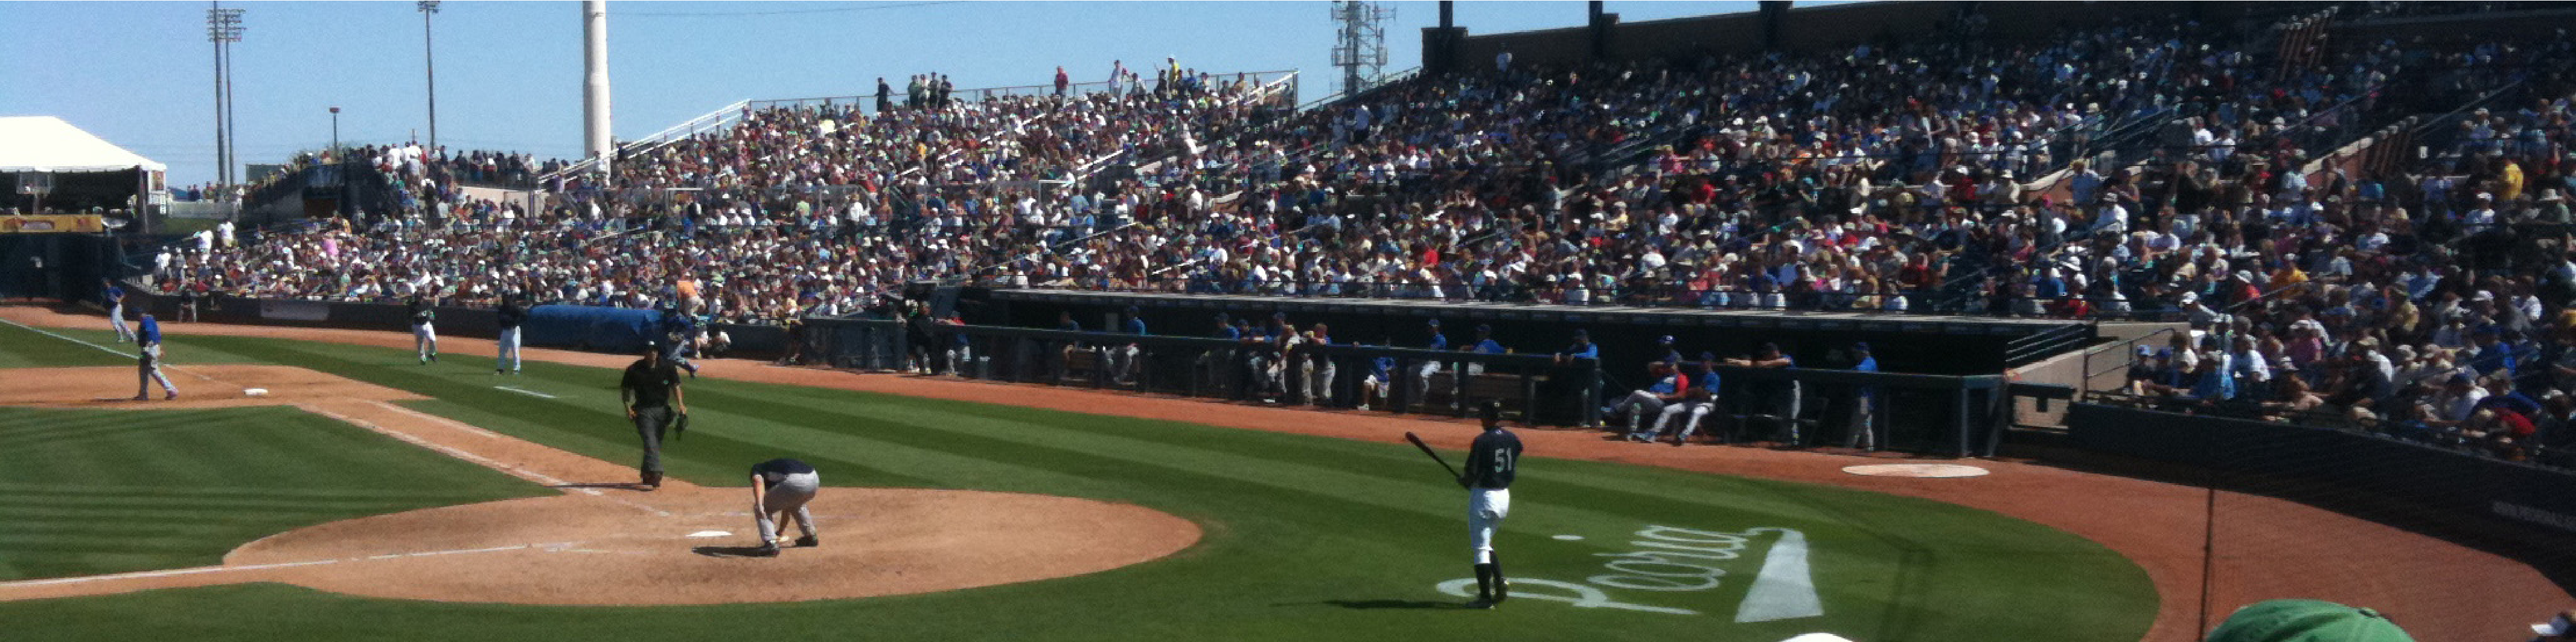
\includegraphics[height=1.5in]{images/sampleteaser}
%%   \caption{Spring Training 2009, Peoria, AZ.}
%% }

\maketitle


\begin{abstract}

Performance of interactive graphics walkthrough systems depend on the time
taken to fetch the required data from the secondary storage to the
main memory. It has been earlier established that a large fraction of this
fetch time is spent on seeking the data on the hard disk. In order to reduce
this seek time, redundant data storage has been proposed in the literature, but
the redundancy factors of those layouts are prohibitively high.  In this paper,
we develop a cost model for the seek time of a layout.  Based on this cost
model, we propose an algorithm that computes a redundant data layout with the
redundancy factor that is within the user specified bounds, while maximizing
the performance of the system.


\end{abstract}



%\begin{CRcatlist}
%  \CRcat{I.3.6}{Computer Graphics}{Methodology and Techniques}{Graphics data structures and data types};
%\end{CRcatlist}

\keywordlist


\section{Introduction}

In typical walkthrough systems, data sets consisting of hundreds of millions of
triangles and many gigabytes of associated data (e.g. walking through a virtual
city) are quite common. Rendering such massive amounts of data requires
out-of-core rendering algorithms that bring only the required data for
rendering into main memory from secondary storage. The time to transfer such data
is known as seek time for our purposes. \\
\\
In this paper, we store redundant
copies of data in order to reduce the seek time. After being given
the data access requirements for a walkthrough application, we develop
an algorithm to duplicate data units strategically to maximize the reduction
in the seek time, while keeping the redundancy factor within the user defined
bound. We show that our greedy solution can generate both the extreme cases
of data layout with redundancy, namely the maximum redundancy case
(a layout where seek time is at most one) and the no-redundancy case (a simple
cache oblivious mesh layout with a potentially high seek time), as well as
reasonable solutions for redundancy factor constraints in between the extremes.
We show that the
implementation of our algorithm significantly reduces average delay and the maximum delay between
frames and noticeably improves the consistency of performance and
interactivity.

\section{Redundancy-based Data Layout Algorithm}

\subsection{Definitions}

There can be many different ways of defining access requirements and data
units. As an example the data units could contain vertices and triangles located near each other and the access requirements would contain the data units required to render a scene from a viewpoint. In general,
the access requirements are determined by the application and are meant to be
sets of data units that are likely to be accessed together. \\
\\
For our seek time model, the
span of an access requirement, number of units between its first and last unit in the linear order, is used as a measure of seek time.
 We assume all access requirements are equally likely to be used thus 
our total Estimated Seek Time (EST) is the sum of the spans of all the access requirements. 


\subsection{Algorithm Overview}

Given the access requirements and the data units, the goal of our algorithm is to compute a data layout that reduces EST.  For our purposes, we are allowed to copy data units, move them, and
delete them if they are not used. Using these operations, we want minimize EST
while also keeping the number of redundant copies as low as possible. 
After we have an initial ordering of data units, we copy one data unit
to another location. We reassign one or more of the access requirements that
use the old copy of the data unit to the new copy making sure the EST is
reduced.  If all the access requirements that used the old copy now use the
new copy of the data unit, then the old copy is deleted, and the data unit was really just moved.  We repeat this
copying and moving of individual data units until our redundancy
limit has been reached. 

\section{Results and Conclusion}

In practice, the performance using the layout with redundancy has generally shorter delays than with the layout without redundancy. Although the layout with redundancy does not eliminate delays , it reduces delays to a small range and keeps the performance more consistent. Additionally, most of these benefits occurred with small redundancy factors. There is a significant improvement in seek time when the redundancy factor is small. However, as you increase the redundancy factor afterward, the improvement in seek time decreases.



%% Use this only if you're preparing a technical paper to be published in the 
%% ACM 'Transactions on Graphics' journal.

\TOGlinkslist

%% Required for all content. 

\copyrightspace

\end{document}
